\documentclass[letterpaper,10pt]{IEEEtran}
\usepackage{geometry}                % See geometry.pdf to learn the layout options. There are lots.
\geometry{letterpaper}                   % ... or a4paper or a5paper or ... 
%\geometry{landscape}                % Activate for for rotated page geometry
%\usepackage[parfill]{parskip}    % Activate to begin paragraphs with an empty line rather than an indent
\usepackage{graphicx}
\usepackage{amssymb}
\usepackage{epstopdf}
\usepackage{multicol}
\usepackage{tikz}
\usetikzlibrary{calc}
\usepackage{mathptmx}
\usepackage{amsmath}
\usepackage{algpseudocode}
\usepackage{url}
\newcommand{\BigO}[1]{\ensuremath{\operatorname{O}\bigl(#1\bigr)}}



\DeclareGraphicsExtensions{.pdf,.png,.jpg}
\usepackage{wrapfig}

% Spacing stuff
\usepackage[cm]{fullpage}
\addtolength{\voffset}{-.5in}
\setlength{\topmargin}{0pt}
\setlength\footskip{0pt}
\setlength{\parskip}{0cm}
%\setlength{\parindent}{1em}
%\usepackage[compact]{titlesec}
%\titlespacing{\section}{0pt}{2ex}{1ex}
%\titlespacing{\subsection}{5pt}{1ex}{2ex}
%\titlespacing{\subsubsection}{0pt}{0.5ex}{0ex}

\title{Mesh Project}
\author{
Donnie Smith (donnie.smith@gatech.edu) \\
Kyle Harrigan (kwharrigan@gatech.edu) 
}	
\date{October 4, 2012}                                           % Activate to display a given date or no date


\markboth{CS 6491 Fall 2012, Project 2}{}
\begin{document}

\bibliographystyle{IEEEtran}

\maketitle

 \begin{abstract}
 
The initial task of Project 2 was the construction of a Delaunay triangulation \cite{wiki:delaunay} of a random set of points using the disk bulge approach and the CLERS \cite{Rossignac99wrapzip} labels of the triangles as they are invaded.  An elegant, concise, and robust algorithm was implemented for the next phase. A short description of the triangulation approach and of how the corner tables (V,S,C) \cite{Rossignac04compressingvolumes} are computed is provided.

Following the construction of the triangulation, the user can click and drag the mouse to define a polygonal curve that may (partially) overlap the mesh.  As the user is drawing it, the program uses that curve to cut the mesh and shrinks the mesh progressively along the cut to give it a realistic look-and-feel.
 
 \end{abstract}
 
\section{"Naive" Exhaustive Triangulation}
\IEEEPARstart{I}{nitially} , a naive triangulation algorithm was implemented to produce the Delaunay Triangulation.  This algorithm is a nested loop over all triplets of points, looking at all combinations.  For each triplet, it computes the Apollonius circle.  It then loops over all other points to determine if they are contained within this circle.  Since this is precisely enforces the condition for the Delaunay triangulation, when it completes it is guaranteed to produce such a triangulation.  

\section{Bulge Triangulation}
A "bulge" triangulation method was also implemented as follows.  The leftmost point is selected as the first vertex (v1).  An imaginary vector pointing directly up is then "swung down" to the right until it encounters the first point.  Mathematically, this is implemented by finding the point which results in the minimum angle between a vector originating at v1 and the vertical and a vector originating at v1 and the test point.  The point which passes this test becomes v2.  
Following this procedure, a recursive bulge process is carried out to the "front" of the segment formed by v1 and v2.    The recursions stops when no points are found "in front" of a side.   

\section{Corner Table Computation}
As each triangulation step adds a vertex, a new triangle is added by adding vertices v1, v2, and the "minimum bulge" vertex v3 to the list of vertices V.  Once a complete list of triangles is computed, C is computed where C[v] is any corner at vertex V by simply looping over the vertices.

\section{Cut Functionality and Logic}
As the cut is drawn through the mesh, intersections are checked at every mouse position update.
When the pointer is outside the mesh, each edge must be checked, but once it enters the mesh, only the three edges of the current triangle need to be checked.
Once a triangle has been entered and exited, it is split into multiple triangles as described in class depending on whether or not the entry and exit points are on the same edge.
It is also possible for the cut to originate and/or terminate inside a triangle, resulting in triangles with a single cut point.
These triangles are split into two triangles separated by a line drawn from the cut point to the opposite corner.

\section{Spreading Method}
In order to spread the mesh away from the cut, all vertices created by the cut are modelled as though they have springs connecting them to the medians of the opposite edges of all triangles using them.
The natural, or forced, length of the spring is one half of the original distance from the vertex to the opposite median.
It should be noted that in this physical simulation, the springs directly change the position, rather than changing the velocity as a true physical force would.
This simplifies the simulation, and avoids oscillations in the mesh.

\section{Results}
As can be expected, the bulge triangulation is orders of magnitude faster than the naive implementation.  In the example case shown on this page, for 15 vertices, only 160 calls were made to the Apollonius solver, whereas the naive method required over 455 calls (appx. 1.84 times more).  For a larger number of vertices (500), the bulge implementation requires only 249,125 calls and the naive implementation requires 20,708,500 calls (appx. 8200 times more).  
The cut functionality works well and provides a real "feeling" as the cut happens. 
\begin{figure}[!t]
\centering
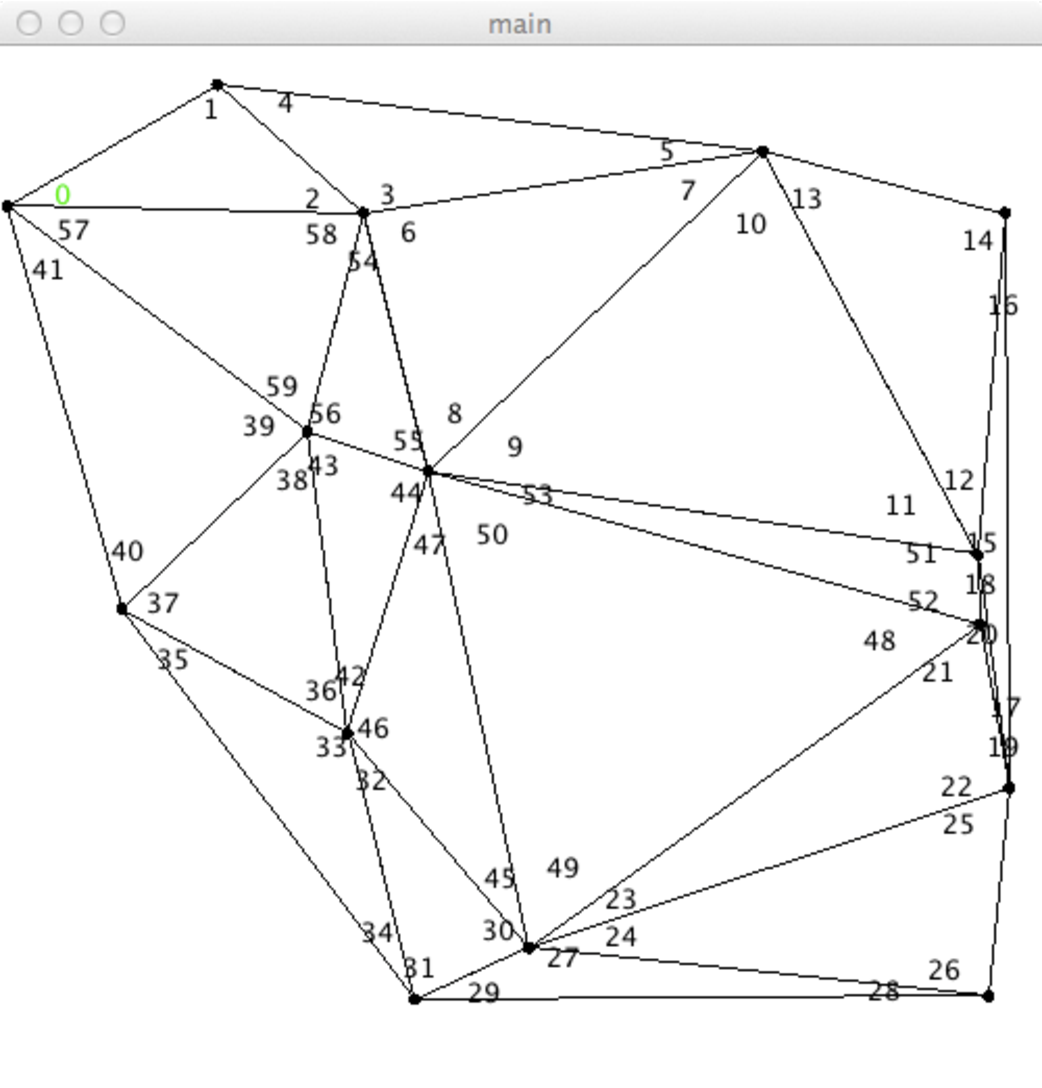
\includegraphics[width=1.75in]{main/data/triangulation}
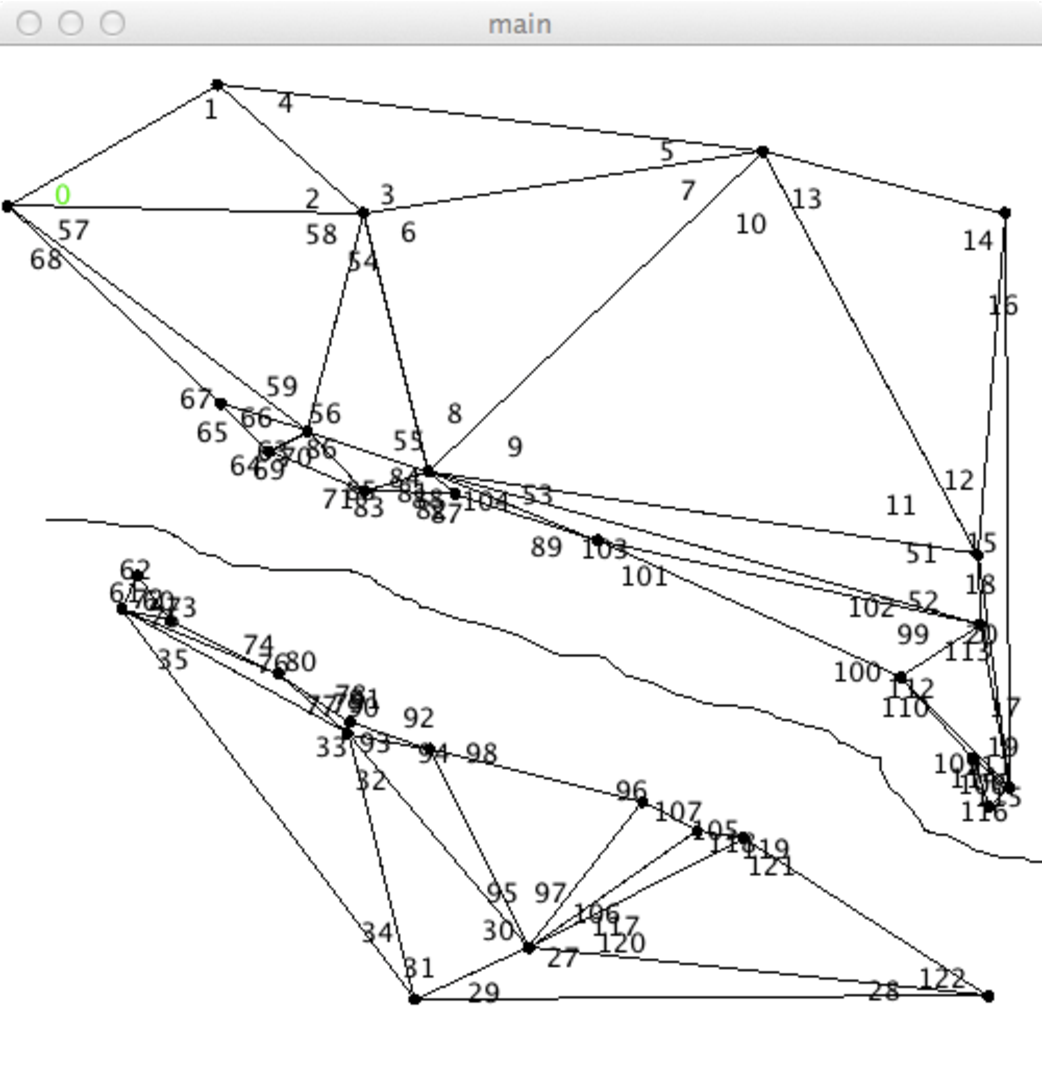
\includegraphics[width=1.75in]{main/data/cut}
\caption{Example Triangulation (left) and a resulting Cut(right)}
\label{fig_triangulation}
\end{figure}

 \section{Conclusion}
 The basic functionality for bulge triangulation, performing a cut, and mesh shrink physics were achieved. 
There are numerous improvements that could be made.  The following is a short list we have thought of:
 \begin{multicols}{2}
\begin{itemize}
\setlength\multicolsep{0pt}
\itemsep0em
\item Improved cut physics by utilizing more complex spring-mass system
\item Implement additional triangulation methods
\item When moving too fast, the cut logic may not function correctly
\end{itemize}
\end{multicols}


\bibliography{cs6491}


%\begin{IEEEbiography}[{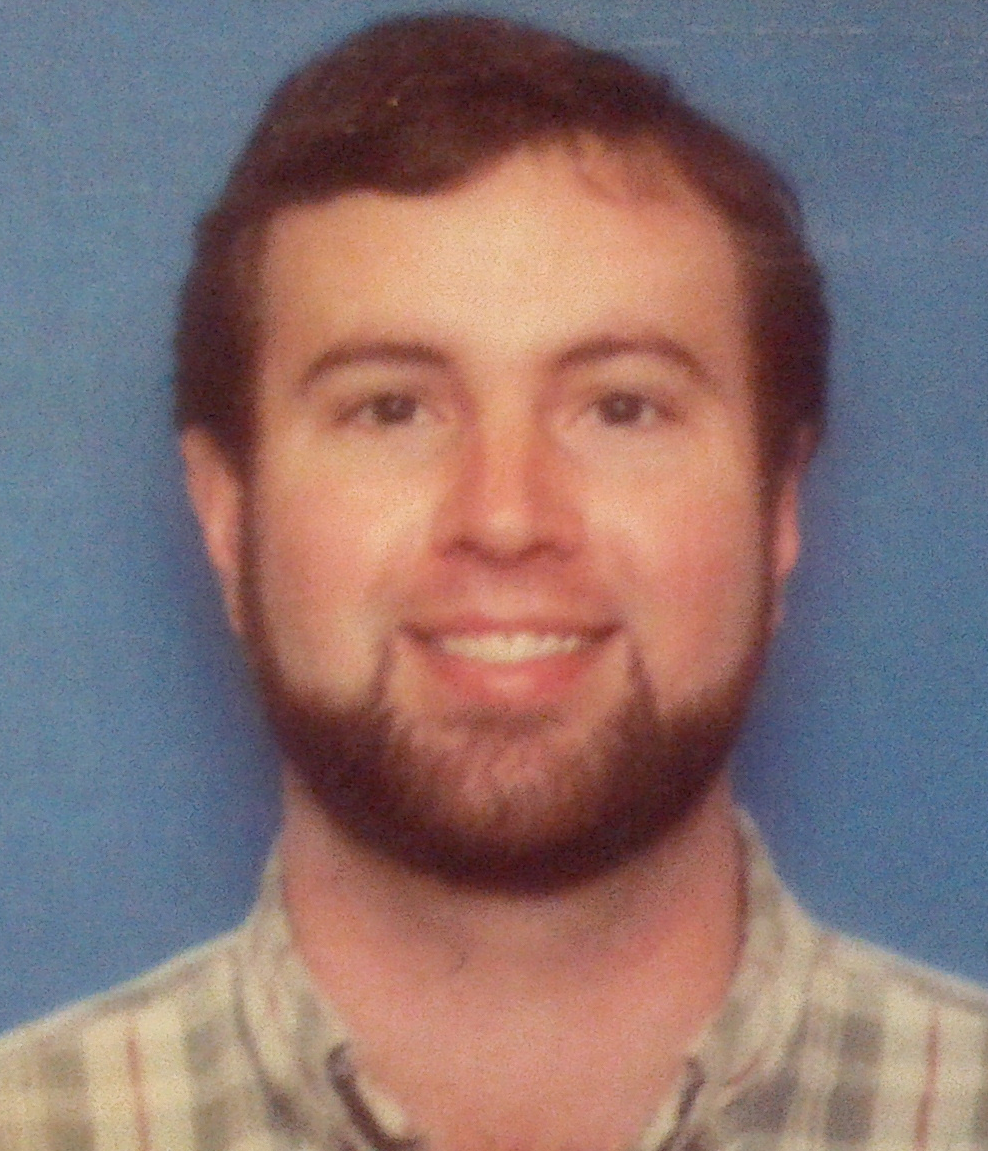
\includegraphics[width=1in,height=1.25in,clip,keepaspectratio]{main/data/dsmith.png}}]{Donnie Smith} donnie.smith@gatech.edu
%\end{IEEEbiography}
%
%\begin{IEEEbiography}[{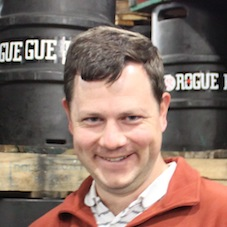
\includegraphics[width=1in,height=1.25in,clip,keepaspectratio]{main/data/kwharrigan.jpg}}]{Kyle Harrigan} kwharrigan@gatech.edu
%\end{IEEEbiography}
\end{document}  



